\begin{figure}[htb]
    \centering
    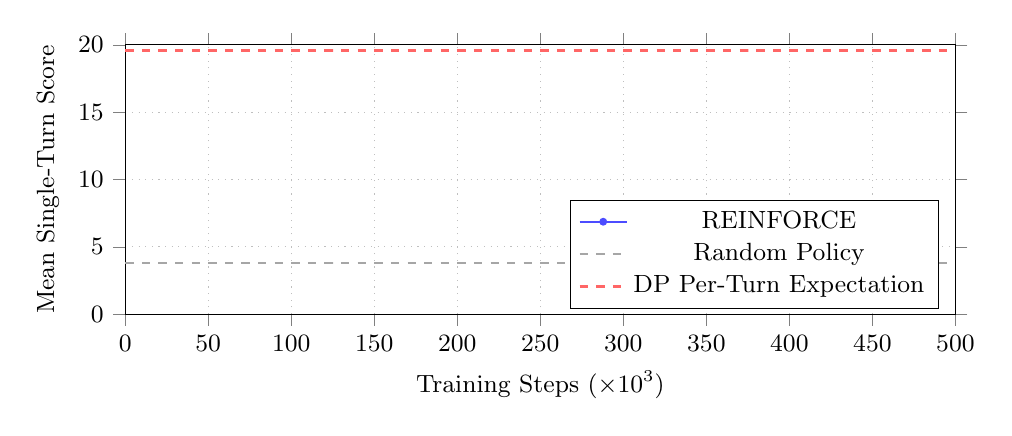
\begin{tikzpicture}
        \begin{axis}[
                width=\columnwidth,
                height=5cm,
                xlabel={Training Steps ($\times 10^3$)},
                ylabel={Mean Single-Turn Score},
                xmin=0, xmax=500,
                ymin=0, ymax=20,
                grid=both,
                grid style={dotted},
                tick align=outside,
                tick label style={font=\small},
                label style={font=\small},
                legend style={at={(0.98,0.02)},anchor=south east,font=\small}
            ]

            % Main REINFORCE learning curve
            \addplot[
                thick,
                blue!70!white,
                mark=*,
                mark size=1pt,
                mark repeat=10
            ] coordinates {
                    (0, 50)
                    (50, 50)
                    (100, 50)
                    (150, 50)
                    (200, 50)
                    (250, 50)
                    (300, 50)
                    (350, 50)
                    (400, 50)
                    (450, 50)
                    (500, 50)
                };
            \addlegendentry{REINFORCE}

            % Random policy baseline
            \addplot[
                dashed,
                gray!70,
                thick,
                domain=0:500
            ] {3.8};
            \addlegendentry{Random Policy}

            % DP per-turn expectation
            \addplot[
                dashed,
                red!60!white,
                thick,
                domain=0:500
            ] {19.59};
            \addlegendentry{DP Per-Turn Expectation}

        \end{axis}
    \end{tikzpicture}
    \caption{Single-turn agent performance during training (placeholder data)}
    \label{fig:single-turn-performance}
\end{figure}
